nEther~\cite{nether} exploits three different attack vectors; CPUID, CPU errata,
and timing information. In this section, we will discuss each attack and
propose our suggested mitigation methods.


\subsection{CPUID Instruction}
\label{sec:approach-cpuid}

Ether alters the output of {\tt CPUID}, flipping the bit for TSC support. This
bit should always be set, both in virtualized and bare metal environment. Can
easily be checked, as shown in Figure~\ref{fig:cpuid-tsc}, in the Appendix.

If it is a bug in the Ether implementation, best solution is to fix, though we
do not have good enough knowledge of the source code to know.

Alternatively, spoof the value in the same manner as {\tt PUSHF} and {\tt POPF}.
Ether deliberately changes the flag register when running, as it sets the debug
flag to be able to step through the target program and get a program trace. It
hides this from the target by spoofing the values of instructions used to read
and write these flags, as {\tt PUSHF} and {\tt POPF}. Figure~\ref{fig:pushf}
shows how the Xen hypervisor is patched to check for specific instructions and
alter the effect of that instruction. The exact same technique could be used to
spoof the TSC-bit when program executes CPUID.

This technique of spoofing the CPUID output suffers from timing attacks, which
will be elaborated in~\nameref{sec:approach-timing}.

\begin{figure}
\begin{lstc}
void vmx_set_pending_exceptions(struct vcpu *v)
{
    ...
+    if(instruction[0] == 0x9C)
+    {
+         /* detected PUSHF */
+
+         v->domain->arch.hvm_domain.ether_controls.send_guest_exception = 1;
+         v->domain->arch.hvm_domain.ether_controls.next_expected_rip = guest_rip + 1;
+    }
+    else if (instruction[0] == 0x9D)
+    {
+         /* detected POPF */
+         ...
+    }
    ...
}
\end{lstc}
\caption{\label{fig:pushf} Part of the patch Ether does on the }
\end{figure}

\subsection{CPU Errata}
\label{sec:approach-errata}

CPU errata refer to the collection of design defects or errors that may induce
the CPU to behave differently from the published specification. Such CPU errata
are strictly bound to a specific CPU model or family that nEther exploits in the
Core 2 Duo family, called AH4 Erratum. The AH4 Erratum states that
"\texttt{VERW/VERR/LSL/LAR} instructions may unexpectedly update the Last
Exception Record (LER) MSR" and there is no planned fix. Concretely,
\texttt{VERW} and \texttt{VERR} instructions verify whether the code or data
segment specified with the source operand is readable (\texttt{VERR}) or
writable (\texttt{VERW}) from the current privilege level. The \texttt{LAR}
instruction loads access rights from a segment descriptor into a general purpose
register, and the \texttt{LSL} instruction loads the unscrambled segment limit
from the segment descriptor into a general-purpose register~\cite{intelsys}.
These errata are design faults, so their existence are unintended. Therefore,
hardware-assisted virtualization solutions (e.g., Xen) will not implement this
erratum in the virtual CPUs of guests, because there is no need to mimic
unexpected system bugs. As a result, malware can detect hardware-assisted
virtualization environments by executing those buggy instructions and, for
instance, checking whether LER MSR is unexpectedly updated. In other words, this
attack cannot recognize the presence of Ether, but can reveal the
hardware-virtualized runtime environment.

The naive solution is patching the buggy instruction in question, or use another
CPU. However, since they are both infeasible we propose two potential solutions;
TODO 1 and TODO 2. \mvf{give a short descriptor to each}

\begin{figure}[!h]
	\centering
	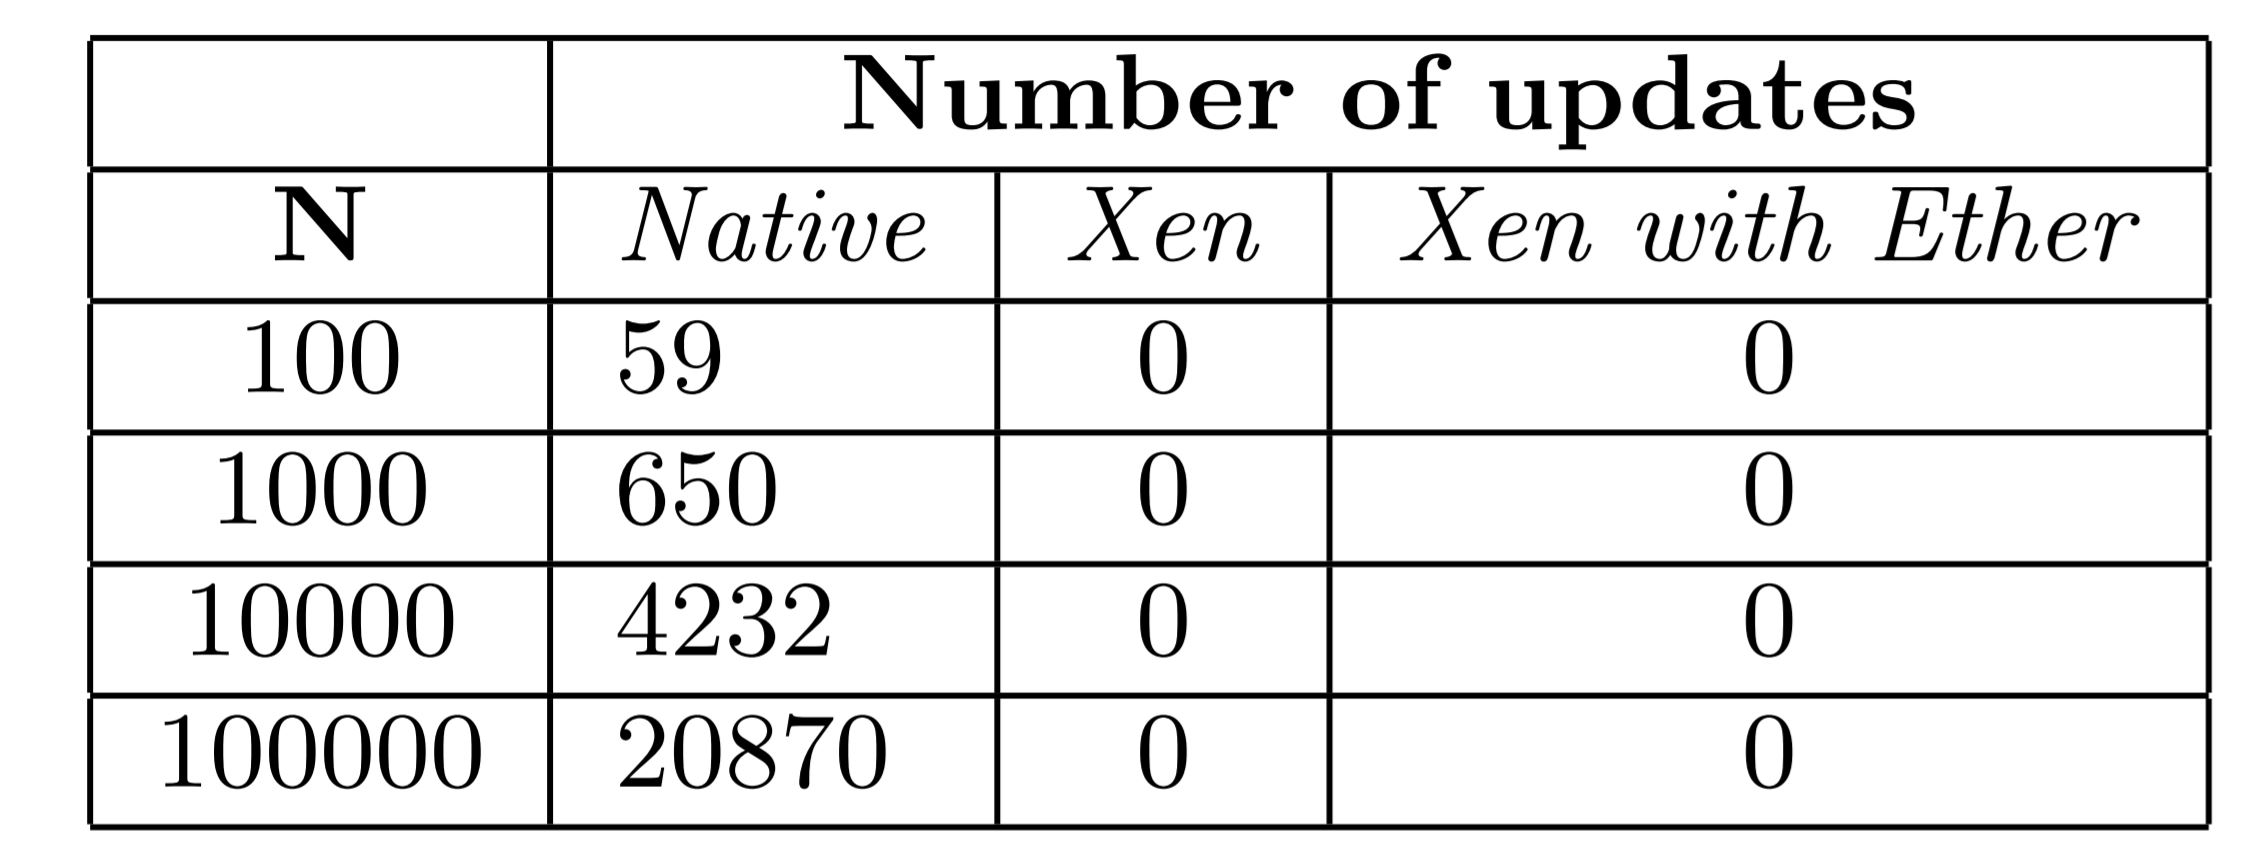
\includegraphics[width=\linewidth]{figure/errata_table.png}
	\caption{The number of LER MSR updates according to the erratum execution}
	\label{fig:errata}
\end{figure}

\subsubsection{Proposed Mitigation 1}
A CPU erratum does not usually occur in normal execution. Table~\ref{fig:errata}
demonstrates the number of LER MSR updates when the CPU erratum was executed
100, 1000, 10000, and 100000 times under the corresponding environments. The
update occurs only in the native environment, but the frequency of occurrences
are unpredictable and irregular (from 20\% up to 65\%). Therefore, the CPU
erratum should be executed several times in order to detect hardware-assisted
virtualization environment. Thus, executing CPU erratum multiple times can be
classified as malicious behavior. To mitigate this, we set a threshold and count
the number of total executions of the known buggy instruction during the runtime
of a program. If the counted number exceeds the threshold, we could either
consider the program as malicious or simply block further execution, depending
on the context of analysis. However, there is a trade-off between true positive
(TP) and false positive (FP) depending on how the threshold is set. Note that
only kernel mode operations can access the LER MSR, and user mode operations do
therefore not need to be blocked nor classified.

\subsubsection{Proposed Mitigation 2}
Another potential mitigation is to intentionally mimic the CPU erratum. The goal
is to hinder the distinction between hardware-virtualized and native
environment. The attack exploits the LER MSR update that only occurs in a native
environment. Therefore, we may mitigate this attack by updating LER MSR
intentionally whenever buggy instructions (\texttt{VERW/VERR/LSL/LAR}) are
executed. This method can be implemented in two ways; the first one is to update
LER MSR directly right after the buggy instruction is executed while monitoring
every kernel mode instruction. Note that we do not need to monitor user mode
instructions, since attack code must be executed in kernel mode in order to
access LER MSR. The second one is to add LER MSR update code right after every
buggy instructions using binary rewriting. LER MSR is divided into {\tt
  MSR\_LER\_FROM\_LIP} and {\tt MSR\_LER\_TO\_LIP}, which are located in {\tt
  0x1dd} and {\tt 0x1de}, respectively. We can add code to modify the value of
{\tt 0x1dd} and {\tt 0x1de} immediately after \texttt{VERW/VERR/LSL/LAR}
instructions, as shown in the Figure~\ref{fig:wrmsr}. Such binary rewriting may
only be conducted only when kernel module is loaded in memory in order to
minimize performance overhead. This mitigation cannot be applied to
self-modifying code, but this is considered out of scope for this paper.


\begin{figure}[h]
\begin{lstc}
__asm__ {
	/* wrmsr : MSR[ECX] = EDX:EAX; */
	...
	verr ax
+	/* store arbitary value in eax, edx */
+	mov ecx, 0x1dd
+	wrmsr 
+	mov ecx, 0x1de
+	wrmsr
	...
	verw cx
+	/* store arbitary value in eax, edx */
+	mov ecx, 0x1dd
+	wrmsr
+	mov ecx, 0x1de
+	wrmsr
	...
}
\end{lstc}
\caption{\label{fig:wrmsr} Code snippet in assembly showing how to rewrite
  a binary for updating LER MSR.}
\end{figure}

\subsection{Timing Information}
\label{sec:approach-timing}
A more sophisticated method of virtualization detection, is taking advantage of
the performance measures and timing information. A virtual machine's performance
will always be slower than it would have been on real hardware, but blindly
measuring the absolute performance scores is not sufficient to detect virtual
environments~\cite{raffetseder2007}. The two approaches are direct comparison of
instructions and caching.

\begin{figure*}[!t]
	\centering
	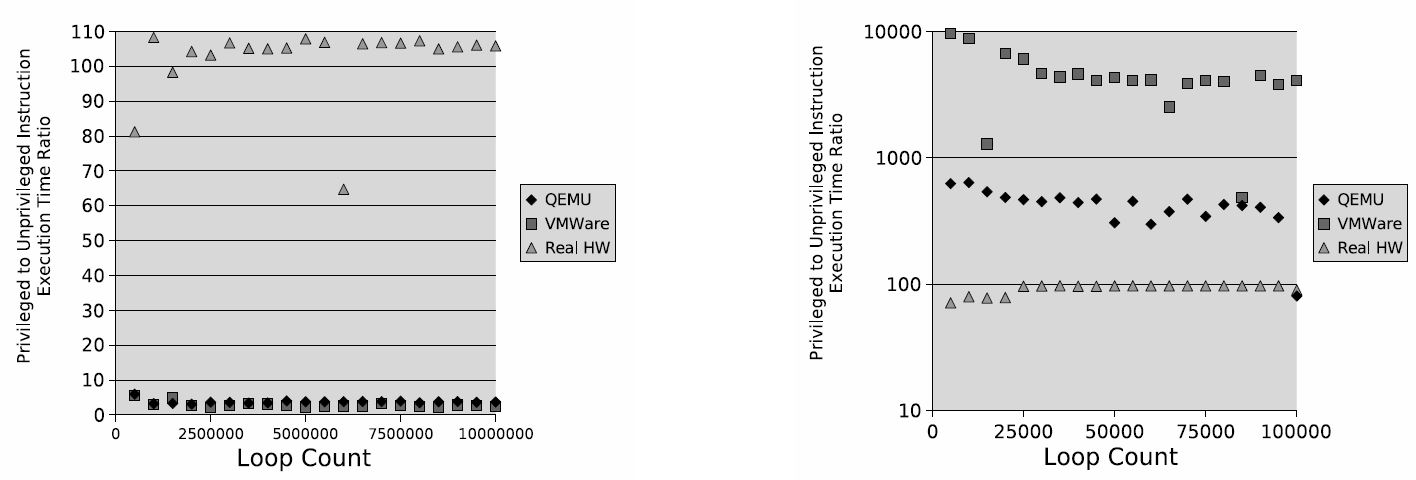
\includegraphics[width=\textwidth]{figure/comp_inst.jpg}
	\caption{Reading/Writing on CR0 (left) and CR3 (right)}
	\label{fig:comparison_of_instructions}
\end{figure*}

\subsubsection{Comparison of Instructions}
Even though a single performance score does not provide any meaningful clues,
comparing the time taken between a privileged and non-privileged instruction can
be useful for detection. Raffetseder {\em et al.}~\cite{raffetseder2007} have
used the performance of non-privileged instructions as a baseline and compared
them to those of a privileged instruction to obtain relative performance numbers.

\begin{equation*}
Relative Performance = \frac{T_{privileged}}{T_{unprivileged}}
\end{equation*}

Real processors have to perform different tasks than emulated processors when
handling privileged instructions. Thus, it causes difference in relative performance
results. Raffetseder {\em et al.}~\cite{raffetseder2007} have conducted an
experiment to prove this concept.  Raffetseder {\em et al.} used the
processor's Time Stamp Counter (TSC) to measure the time elapsed to execute an
instruction, as shown in Figure~\ref{fig:comparison_of_instructions}. Real
hardware showed poor relative performance when accessing {\tt CR0}, but greater
performance when accessing {\tt CR3}. Although Raffetseder {\em et al.} did not
explicitly explain why the results differed in terms
of 10 to 100 times between emulated and real environments. The difference is large enough to detect virtual
environments.

\subsubsection{Mitigation of Comparison of Instructions}
\label{sssec:mitigation_relative}

Raffetseder {\em et al.}'s~\cite{raffetseder2007} experiments on comparison of
instructions were done on software-based emulation solutions (e.g. Qemu, VMware,
etc.) which are buggy and fundamentally more limited than hardware solutions
(e.g. Intel VT-x, AMD-V). Intel VT-x, that runs on the Xen hypervisor, provides
the \texttt{TSC\_OFFSET} (Time Stamp Counter Scaling Offset) field additional to
the regular \texttt{TSC} field that is specifically designed to skew the guest
time upon clock cycle request. When the guest queries for the \texttt{TSC}
value, the hypervisor will return the \texttt{TSC} minus the
\texttt{TSC\_OFFSET}. Since the \texttt{TSC\_OFFSET} is under control of the
hypervisor, sandboxing the malware on hardware-based virtual environment should
mitigate the relative performance difference vulnerability.

\subsubsection{Cache-based Detection}
Caching lets the system hold on to recently executed instructions in case they
are needed again in near future. As a result, executing cached functions will
require less CPU cycles compared to the first time as shown on
Figure~\ref{fig:cache_realhw} left. However, caching can be turned off on
machines running on bare metal by making the processor enter the no-fill cache
mode and flushing out all existing caches by using the {\tt WBINVD} instruction.
As a result, latter executions consume the same amount of CPU cycles as the
first run, as shown on Figure~\ref{fig:cache_realhw} right. However, it was
shown that disabling caching is not properly supported on Qemu and VMware.
Raffetseder {\em et al.}~\cite{raffetseder2007} have executed six independent
test runs where each test run consists of five calls to one function. Both Qemu
(Figure~\ref{fig:cache_qemu}) and VMware (Figure~\ref{fig:cache_vmware}) had
significant CPU cycle reduction after the first execution regardless of the
caching preference. Therefore, malware authors can take advantage of the fact
that caching cannot be disabled on virtual environments. If a malware obtain
measurements similar to Figure~\ref{fig:cache_qemu} or
Figure~\ref{fig:cache_vmware}, it should consider itself being run in a sandbox
and hide its malicious behavior. The malware authors can also take advantage of
TLB flush to detect virtualization. As mentioned in
\ref{sssec:mitigation_relative}, software based solutions are buggy and
fundamentally limited to provide good virtualization, thus it is easy for
malware to detect them. Malware analyzers running on top of hardware assisted
virtualization can trigger TLB flush to emulated caching being disabled. When a
context switch is made from the guest to the hypervisor, the TLB is flushed to
change the guest's context to that of the hypervisor. Since a TLB flush can be
triggered by using non-privileged instructions \footnote{trapped down to the
  hypervisor and also available in the guest}, the time taken by an instruction
can be calculated by running code similar to that shown in
Figure~\ref{fig:cache_mitigation}. Upon calling non-privileged instructions that
should cause the TLB to be flushed, the time taken will decrease if the TLB has
not been flushed. However, the TLB has been flushed, then the time will
increase.

\subsubsection{Mitigation of Cache-based Detection}
Controlling low level CPU caching is very difficult due to the complexity of
modern chaches, which are up to 8-way set associative etc. Thus, attempting to
fill up cache is not an easy job. There is no good known solution to preventing
cache-based detection. Theoretically, Address Space Identifier (ASID) prevents
the need for TLB flushing, however, it is difficult to use it effectively on low
level cache.

\begin{figure}[h]
\begin{lstasm}
; calc mean time before
loop:
	retsc
	;; test
	rdtsc

; flush tlb
cpuid

; check time after
rdtsc
;;test
rdtsc

; very different? 
cmp $before $after
\end{lstasm}
\caption{\label{fig:cache_mitigation} example code to measure the mean running
  time of an instruction.}
\end{figure}


%%% Local Variables:
%%% mode: latex
%%% TeX-master: "../paper"
%%% End:
